\documentclass[a4paper,12pt]{report}
\usepackage{amsmath}
\usepackage{graphicx}
\usepackage[utf8]{inputenc}
\usepackage{amssymb}
\usepackage{color}
\usepackage{CogSciBScUOS}
\usepackage{indentfirst}
\usepackage{enumitem}
\setlist{nosep}
\graphicspath{ {Examples/} }



\title{Automatic Prediction of Harmonic Rhythm from Melodies}
\author{Valentin Huemerlehner}
\email{vhuemerlehne@uni-osnabrueck.de}
\firstSupervisor{Prof. Dr. Kai-Uwe Kühnberger}
\secondSupervisor{PhD Maximos Kaliakatsos-Papakostas}


\begin{document}

\beforepreface %needed clause, generates e.g. title page

\prefacesection{Abstract}
In this thesis, I tried to predict a valid and most likely harmonic rhythm of a given melody according to the harmonisation of a specific style. Annotated to the melody are cadences and the information on bar boundary placement. Conditional probabilities for harmonic rhythmic events were extracted from thoroughly annotated melodies: They had harmonic reductions of the actual accompaniment given alongside the melody, allowing for a comparison between idioms and how strongly they differ as well as extraction of correlations between melody and harmonic rhythm. From the regularities found in the second step, the harmonic rhythm of melodies not included in the analysis was predicted and compared to the actual harmonic rhythm occurring in the piece.

\prefacesection{Acknowledgements}
I want to thank a number of people for their direct or indirect help in creating this work:

Firstly, my parents for giving me absolute freedom of choice in all decisions, yet always being available for advice when needed.

My friends who actually made me work by working in a group at the same time. They may not have known, but they were absolutely pivotal.

Anne Dominique. No explanation needed.

The more musically, computationally or Englishly inclined friends who read and criticised the thesis for improvements.

Prof. Kühnberger for input and ideas, especially in terms of evaluation.

Prof. Cambouropoulos and Prof. Tsougras for their musicological insights and literature help.

Maximos Kaliakatsos-Papakostas for almonds, advice, Matlab support and much more. You basically made this thesis possible singlehandedly and additionally made the time in Thessaloniki not only productive, but also highly enjoyable. Thank you especially!

\afterpreface %needed clause, generates e.g. table of contents
\newpage

\listoffigures
%\newpage

\pagenumbering{arabic}

\chapter{Concurring ideas on computational creativity}
In the last years, scientific progress on computational creativity has accelerated more and more in all aspects of creativity. In the fine arts, this progress is mainly driven by neural networks, allowing for new techniques such as style overlaying or style blending and recombination of different aspects of an image (such as form and texture). In music, neural networks were for a long time not able to outperform other techniques, but they are beginning to make their mark, one example being ``DeepBach", a neural network able to copy Bach's chorale style (or any other, provided the correct input) and already fooling even musical experts at a decent rate\footnote{\cite{hadjeres2016deepbach}}.

One example for a more hands-on approach is the CHAMELEON harmonising system created at the Aristotle University Thessaloniki by Kaliakatsos-Papakostas, Makris, Zacharakis, Tsougras and Cambouropoulos.\footnote{\cite{kaliakatsos2016overview}} I wrote this thesis in its context, thus I will explain the system's workings briefly. For a more detailed description, you may want to have a look at the extensive paper.\footnote{\cite{kaliakatsos2016learning}}

\newpage
\section{The CHAMELEON harmonising system}
\begin{figure}[h]
\centering
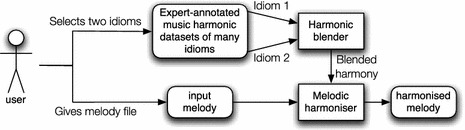
\includegraphics[scale=0.7]{Chameleon_overview.jpg}
\caption{Graphical overview over the CHAMELEON harmonising system}
\end{figure}


\chapter{Musictheoretical background}
\section{General western music theory}
As this thesis exists mainly in the context of Artificial Intelligence and Cognitive Science, I will give a brief overview on western music theory necessary for proper understanding of the later parts. However, this introduction presupposes the understanding of musical notation. If you do not know how to read music or would like to remind yourself of it, there are plenty of tools available online\footnote{E.g. the WikiHow explanation at http://www.wikihow.com/Read-Music} or in print.\footnote{E.g. \cite{cooper1982read}} If you feel comfortable with the notions of western music notation, meter, rhythm, intervals, harmony, harmonic functions and scale degrees, especially in the context of a Roman numeral analysis, I encourage you to skip ahead. Else, the following introduction that closely follows Walter Piston's book "Harmony", chapters 1, 2, 5 and 11,\footnote{\cite{piston1987harmony}} should provide you with the necessary basics.

\subsection{Intervals, scales and harmonies}
\subsubsection{Intervals and scales}
The tonal distance between two notes, successive or simultaneous, is called interval. If the two notes sound simultaneously, the interval is called harmonic, if they are heard one after the other, it is melodic. Beware that also the same note repeated is called an interval, the unison. Below is a complete list of all general interval names up to one octave. They are defined by the distance in number of lines and spaces in the staff.\footnote{\cite{piston1987harmony}, p. 7}

\begin{figure}[h]
\centering
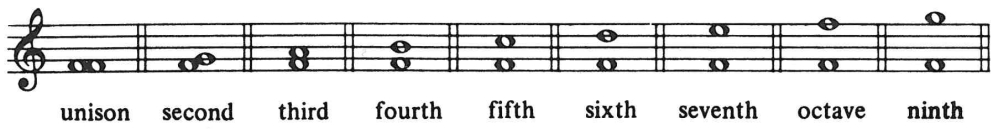
\includegraphics[scale=0.32]{Piston_1.jpg}
\caption{Interval names}
\end{figure}

The further classification of intervals refers to scales, specifically the two most common ones in western tonal music (also referred to as "common-practice" music): major and minor. Below you can find the C major and C natural minor scales, i.e. the two scales starting on the note C.\footnote{\cite{piston1987harmony}, p. 5}

\begin{figure}[h]
\centering
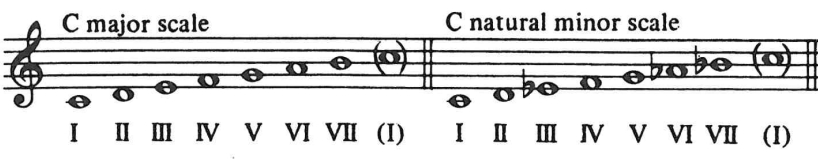
\includegraphics[scale=0.35]{Piston_2.jpg}
\caption{Natural major and minor scales on C}
\end{figure}

The precise interval name can then be found by imagining each scale on the lower of the two notes in question. If the upper note happens to lie within the major scale, it is called \textit{major}, if it lies in the natural minor scale, it is called \textit{minor}. Imagining these two scales overlapping, you can notice that unison, fourth, fifth and octave conincide. Thus, these intervals instead receive the prefix \textit{perfect} whenever they occur. This leaves some intervals to be named. If a major or perfect interval is made larger by one semitone, it is then called \textit{augmented}. If however a minor or perfect interval is made smaller by one semitone, it is then called \textit{diminished}, as can be seen below.

\begin{figure}[h]
\centering
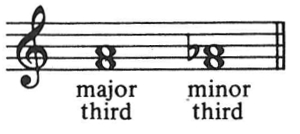
\includegraphics[scale=0.45]{Piston_3.jpg}
\caption{Major and minor intervals}

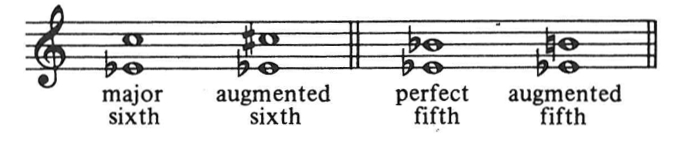
\includegraphics[scale=0.4]{Piston_4.jpg}
\caption{Augmented intervals}


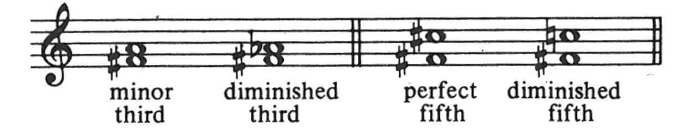
\includegraphics[scale=0.4]{Piston_5.jpg}
\caption{Diminished intervals}
\end{figure}

\subsubsection{Chords and Harmonies}
Sounding two or more intervals at the same time forms a chord. In common-practice, most chords are based on two thirds, forming a \textit{triad} of notes. The lowest note is then called \textit{root}, the other two \textit{third} and \textit{fifth}, according to their distance to the root. These names are fixed independent of the arrangement. Thus, a triad may be inverted, leaving the root in a position other than the lowest tone. Still, whenever the three notes may be positioned in a way that they form two thirds, this defines the root.

Depending on the kinds of thirds used, there are four possible combinations and differently sounding kinds of triads:

\begin{center}
	\begin{tabular}{|l|c|r|}
		\hline
		\textbf{Lower third\textbackslash Upper third} & \textbf{Major} & 			\textbf{Minor}\\ \hline
		\textbf{Major} & Augmented & Major\\ \hline
		\textbf{Minor} & Minor & Diminished\\ \hline
	\end{tabular}
\end{center}

\subsection{Harmonic functions and Roman numeral analysis}
In different contexts, the same chord may have be heard extremely differently and may have a wide range of emotional valences. Building triads of only the notes that lie within a major scale on all notes that lie within the scale, we can give these chords names and symbols, specifically Roman numerals depending on the position within the scale\footnote{\cite{piston1987harmony}, p. 13}:

\begin{figure}[h]
\centering
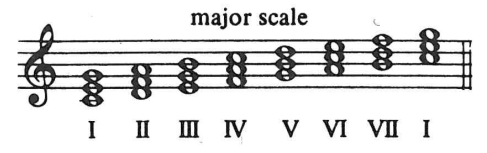
\includegraphics[scale=0.4]{Piston_6.jpg}
\caption{Roman numerals on a C major scale}
\end{figure}

Most of these are of no further importance to this thesis, but the three basic harmonic functions are. They are I (or i in minor mode), IV and V, also called \textit{tonic}, \textit{subdominant} and \textit{dominant}. The tonic builds the basis of tonal music, in common-practice building a piece's frame by standing at the beginning (very rarely preceeded by a dominant to signify strong movement) and the end of a piece. The dominant is used as a creator of tension, generating a sense of necessity to return to the tonic. Almost always, the point of highest harmonic tension in a piece contains the use of one or more dominants. This can be achieved by hierarchically layering and relabelling the functions: a dominant chord may itself be preceeded by its own dominant chord and so forth. The subdominant can be seen as creator of movement and diversity in common-practice music. It is not strictly necessary for a closing cadence (as can be seen in many examples of classical as well as folk music), but generally, its usage will yield more interesting results.

\subsection{Cadences}
As mentioned above, the dominant is often used as point of maximal tension, thus providing an excellent penultimate chord that is then resolved into the tonic. This progression is called an \textit{authentic cadence} because for most western listeners, it provides the strongest sense of satisfying closure.
\begin{figure}[h]
\centering
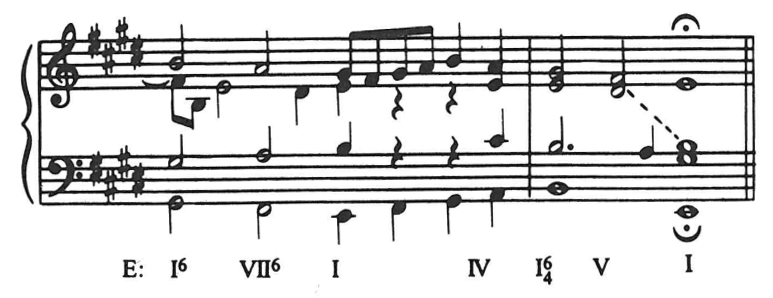
\includegraphics[scale=0.4]{Piston_7.jpg}
\caption{Authentic Cadence - J.S. Bach: \textit{Well-Tempered Clavier, II, Fugue No. 9}}
\end{figure}

In a special case, where the two chords appear in root position -- i.e. with the root as the lowest note -- and the most prominent (most of the time highest) voice ends in the tonic note, this authentic cadence is called \textit{perfect cadence}. In all other cases, it is called \textit{imperfect}.

Another type of cadence is the \textit{plagal cadence}. It also ends in the tonic, but its penultimate chord is the subdominant. It generally has a slightly archaic feeling to it, since its usage was more common in renaissance music, standing on the verge between modal and tonal music.
\begin{figure}[h]
\centering
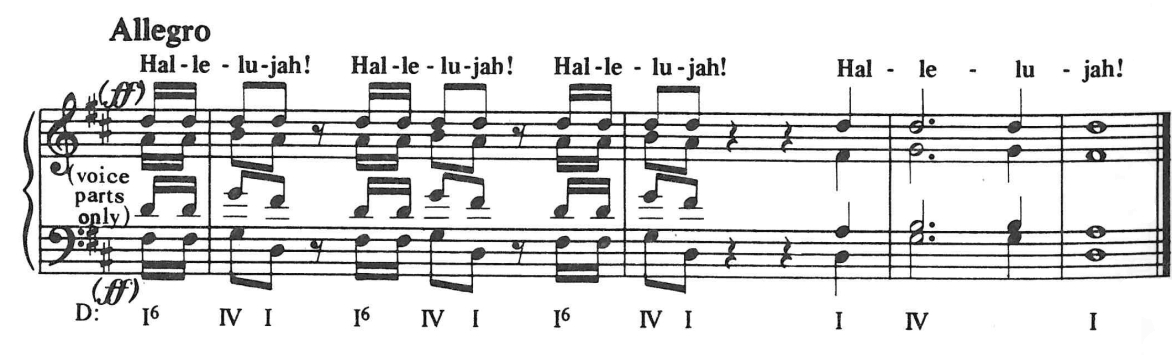
\includegraphics[scale=0.35]{Piston_8.jpg}
\caption{Plagal Cadence - G.F. Händel: \textit{Messiah, Hallelujah Chorus}}
\end{figure}

These cadences may be used in such a way that the last chord is on the downbeat or that the second to last one lies there, resolving on a less significant beat, thus implying the penultimate chord's higher significance.

With this introduction I hope to have covered all necessary terminology and concepts, but for a deeper understanding, I highly recommend further study of the topic, e.g. in form of books and online classes -- or, if you have the money, private lessons.

\section{Harmonic rhythm}
When thinking about harmonic rhythm, I ran into the problem of a lacking common definition in the literature. Therefore, I will give a historical overview on the topic.

\subsection{First formal definition by Walter Piston}
\subsubsection{Harmonic rhythm in practice}
For the longest time, harmonic rhythm was a concept that was only roughly outlined, yet left untouched in terms of a precise definition. Jean Philippe Rameau -- the first western composer to properly write down some of the existing concepts of "good" compisition practices -- only states that one should not change harmony on the weak beats of a bar.\footnote{\cite{rameau1722traite}, book 3, chapter 40, p.317f.} This concept was agreed upon quite commonly, showing that in practice, composers were well aware of the effect that harmonic changes, meter and their interaction had.
\subsubsection{Definition as root changes}
Yet, it was not until 1944 that Walter Piston tried to give a more formal definition of harmonic rhythm in the first edition of the Harvard Dictionary of Music:
\begin{quote}
Harmonic rhythm. The rhythmic life contributed to music by means of the underlying changes of harmony. The pattern of the harmonic rhythm of a given piece of music, derived by noting the root changes as they occur, reveals important and distinctive features affecting the style and texture.\footnote{\cite{willi1944harvard}, as cited in \cite{swain2002harmonic}, p.6}
\end{quote}
He elaborates on this definition in his book "Harmony".\footnote{\cite{piston1987harmony}, read in the 4\textsuperscript{th} edition edited by Mark DeVoto, 1978} In this volume, he strongly presupposes a western tonality in the sense of a Roman numeral analysis of harmonies. Using a harmonic analysis of a given piece, he then defines root changes as the rhythmic events that make up harmonic rhythm.\footnote{[ibid.], p.190f.} Thus, melodic and harmonic rhythm may, but do not necessarily have to coincide (a possible example of parallel harmonic and melodic rhythms are homophonic passages, where all voices or instruments progress melodically at the same time, often leading to harmonic progression).\footnote{[ibid.], p.191ff.}

\subsubsection{Frequency of root change}
A perceptually highly salient aspect of harmonic rhythm is the general speed of harmonic movement.\footnote{[ibid.], p.193ff.} As can be seen in the two examples, the range of possible tempi is large. Even the complete lack of harmonic changes may be applied to great effect, although in many cases, such a missing sense of movement is perceived as bland. A special case of a static harmonic rhythm can be a bass pedal -- i.e. a single note that is held or repeated over a prolonged period of time, to some degree independent of the other voices' development -- that ''[...] tends to overpower the sense of harmonic progression[...]''.\footnote{[ibid.], p.196} Hence, even though movement may be present harmonically, it is perceptually omitted by the stronger effect of the pedal.

\subsubsection{Strength of harmonic progressions}
As one might expect -- and for the purpose of this work quite unfortunately -- the perceptual importance of harmonic changes is not independent of their content, i.e. the actual change applied.\footnote{\cite{rameau1722traite}, book 3, chapter 40, p.315f. and \cite{piston1987harmony}, p.196f.} A prime example for an especially salient progression -- at least in western music -- are cadences that provide closure after a point of maximal tension.\footnote{For theoretical insights, see -- among many others -- \cite{jackendoff1983generative}, for experimental evidence, see \cite{bigand1999perceiving}.} As already seen in Rameau's treatise, the rhythm and timing of these progressions used to be highly regulated. While such rules weakened and to a certain degree disappeared in the late 19\textsuperscript{th} and beginning 20\textsuperscript{th} century,\footnote{For rather conservative views on harmonic rules, see \cite{riemann1893vereinfachte} and \cite{schenker1906harmonielehre}. For the highly progressive view of Arnold Sch\"onberg, albeit before development of his twelve-tone theory, see \cite{schonberg1922harmonielehre} and for an example of complete deletion of harmonic considerations, see \cite{schonberg1976stil}.}, they might still give an important hint towards the positioning of harmonic changes, justifying a trial to find most likely beats for harmonic changes within a meter.

\subsubsection{Dynamic indications}
According to Piston, the harmonic rhythm and its valence may also be influenced by dynamic indications made by the composer to clearly indicate their intentions, possibly overriding the interpreter's musical intuitions.\footnote{\cite{piston1987harmony}, p.198f.} However, since this phenomenon of contradicting information from musical intuition and compositional indications is somewhat rare, I did not include it in my analyses.

\subsubsection{Nonharmonic chords}
Lastly, Piston also postulated the existence of nonharmonic chords, similarly to nonharmonic notes. Nonharmonic chords are those that, despite presenting a root change and thus some harmonic movement, are not processed as such by the listener.\footnote{[ibid.], p.201} This mostly occurs in fast passages where movement is abundant and is facilitated by the chords not being presented in root position, thus omitting the root note and hindering recognition of the chord. This again is an infrequent phenomenon, which I left out in my analysis. It is however a candidate for future expansion.

\subsection{Enhancements of Piston's work}
\subsubsection{Problems about the root change approach}
The main problem about Walter Piston's approach to harmonic rhythm is that an analysis in the form of Roman numerals needs to exist. This actually entails two separate problems: On the one hand, such an analysis has to be possible in the first place, i.e. the music needs to be tonal for it to properly work. This is not the case for all music predating the renaissance, for quite a range of music (Twelve-tone Music, Experimental Music, Rock, Metal, etc.) starting from the 20\textsuperscript{th} century and most music that does not stem from the European tradition. On the other hand, analyses of this kind do not always follow strict rules, but involve the analyser's interpretation of certain ambivalent occurences (e.g. an underdefined harmony, where only two notes of a triad are played and thus, multiple triads could fit). One example where this was criticised, but not circumvented, is the article "Harmonic Rhythm in Beethoven's symphonies" by Jan LaRue \footnote{\cite{la2001harmonic}}. The other details of the article are of no interest to this thesis (although quite interesting from a musicological point of view).

\subsubsection{A solution proposed by Joseph Swain}
This exact problem of ambiguity is tackled in Joseph Swain's book with the telling title ''Harmonic Rhythm - Analysis and Interpretation''. Swain sees himself in Piston's tradition and thinks of his work as a mere consequence: \begin{quote}There is no reason to think that Walter Piston would disapprove of such hierarchical pictures. They are logical extensions of his original insight.\footnote{\cite{swain2002harmonic}, p.57}\end{quote} He introduces a hierarchical system of analysis levels that form around Piston's central idea of root changes in a moderate -- i.e. processable -- speed. I will introduce the different levels of analysis under the point of view of utility and feasability in the following.

\subsubsection{Rhythm of the texture}
Swain's first level of analysis is the rhythm of the texture. It is produced by simply adding up all rhythmical events into a single line, thus denoting all rhythmical events the listener could possibly perceive.\footnote{[ibid.], p.15ff.} This means that at any harmonical rhythmic event -- no matter the exact definition -- needs to necessarily correspond to a textural rhythmic event.\footnote{[ibid.], p.17} However, there are easily imaginable examples for textural rhythmic events that can not be counted as harmonic rhythm since no change in pitches occurs. One example are repeated chords, as found in the Triple Concerto op. 6, No. 3 by Arcangelo Corelli\footnote{\cite{swain2002harmonic}, p.18}. In this excerpt, we can also see the problem that textural rhythm following Swain does not differentiate between voices This leads to many more textural events than harmonic events (taking the Ripieni strings as indication for harmony). Hence, I did not include textural rhythm in my analysis.
\begin{figure}[h]
\centering
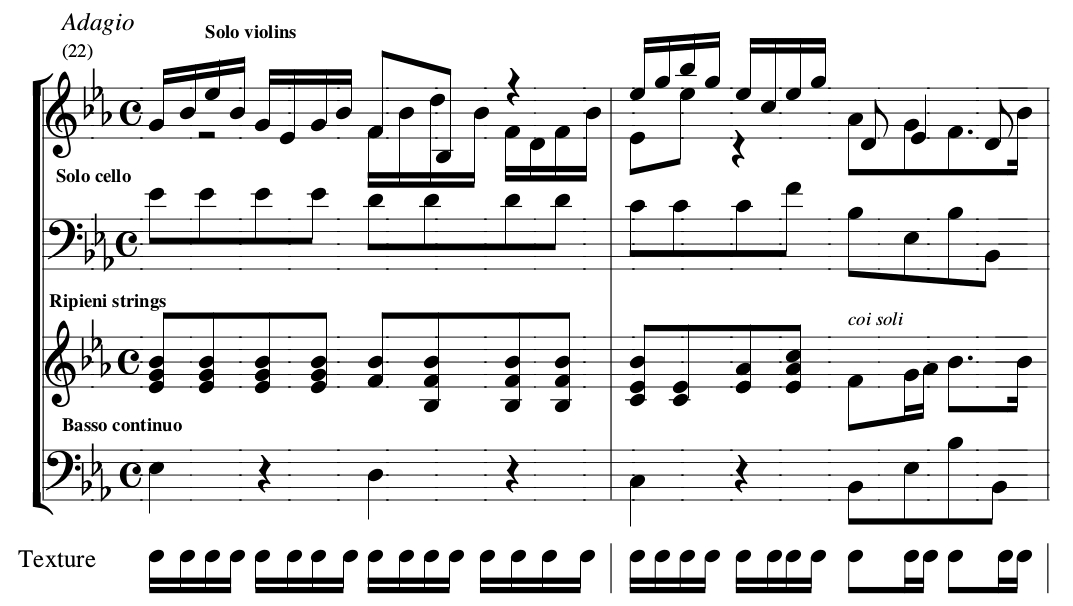
\includegraphics[scale=0.35]{Corelli_triple_concerto.jpg}
\caption{Textural rhythm - A. Corelli: \textit{Triple Concerto for 2 Violins and Violoncello, op. 6 No. 3}}
\end{figure}


\subsubsection{Phenomenal harmonic rhythm}
The next dimension is called the phenomenal harmonic rhythm. It denotes all time points at which the chord changes in any way, including new harmonies as well as inversions of chords. Quite often, textural and phenomenal harmonic rhythm may be the same, but a prominent example of the opposite can be seen in the beginning of Antonio Vivaldi's fourth concerto of the so called "Four Seasons" (op. 8, no. 4, "Winter", I)\footnote{\cite{swain2002harmonic}, p.23}:

\begin{figure}[h]
\centering
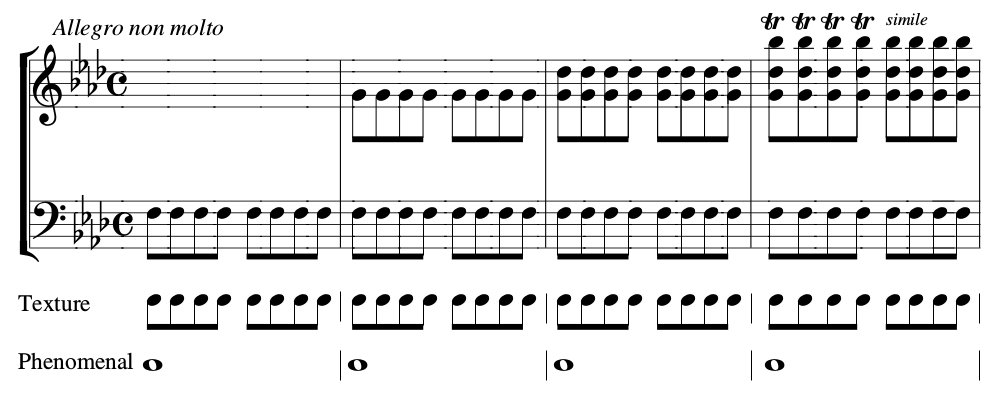
\includegraphics[scale=0.35]{Vivaldi_four_seasons_winter.jpg}
\caption{Textural and phenomenal rhythm - A. Vivaldi: \textit{Concerto grosso op. 8, no. 4, "L'inverno", I}}
\end{figure}

Swain further differentiates between this texture phenomenal harmonic rhythm and what he calls contrapuntal phenomenal harmonic rhytm. The latter he defines as follows: "the changes in harmonic phenomena caused by moving voices."\footnote{[ibid.], p.28} The concept is easiest to understand by virtue of an example\footnote{\cite{swain2002harmonic}, p. 25}:

\begin{figure}[h]
\centering
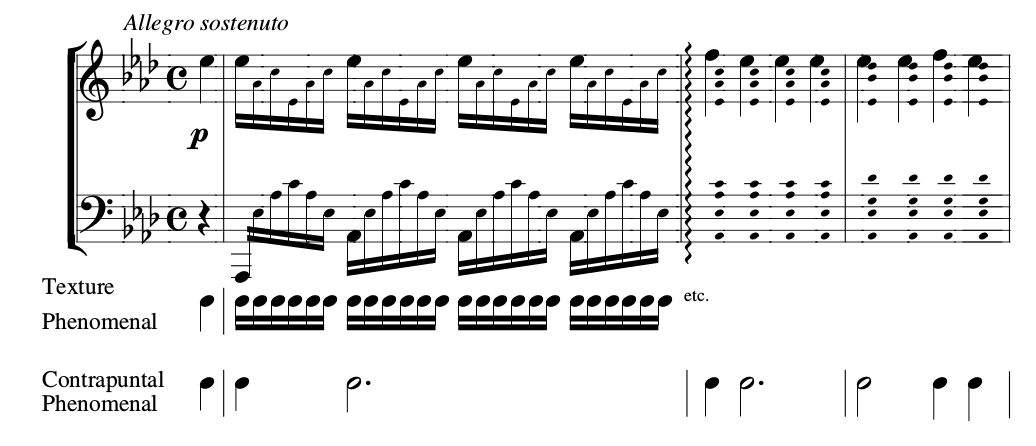
\includegraphics[scale=0.35]{Chopin_etude_25_1.jpg}
\caption{Texture phenomenal and Contrapuntal phenomenal harmonic rhythm - F. Chopin: \textit{12 Etudes, op. 25, no. 1}}
\end{figure}

In Fr\'{e}d\'{e}ric Chopin's \'{E}tude op. 25, no. 1 for piano, bass and melody are played in the respective outside fingers of each hand while the other fingers contribute the harmonies in the form of rapid arpeggios. These do count into the textural phenomenal harmonic rhythm, but are not a separate voice in Swain's definition, thus not being included in the contrapuntal version. The differentiation therefore seems to be one of perceptual relevance: The middle parts are not perceived as melodic events due to their high speed and dynamical softness and therefore are not part of the counterpoint.

To check for the importance of phenomenal harmonic rhythm for the purpose of this thesis, I will take a look at Swain's reasoning: According to him, a comparison between textural and phenomenal rhythm can already provide first insights into the emotional valence of a passage, which however is of no further interest in my case. More interestingly, he sees this level of analysis as the only one to remain free of an evaluation of harmonic events:\footnote{[ibid.], p.23} Since every (perceived) change in pitches is denoted, the content of the change is not important, but the two harmonic events before and after the change can be compared neutrally. This makes this level of analysis interesting for non-tonal (ancient and modern) as well as non-western music. In the corpus of pieces used for this thesis, only tonal and western music was used, which makes this level obsolete, but for a more general solution to the problem, its inclusion may be necessary.

\subsubsection{Bass pitch harmonic rhythm}
On the next level, Swain examines the changes in the bass voice. Notably, the bass voice need not necessarily always be the lowest voice. Part-crossings due to voice-leading considerations and timbre may lead to the lowest note not being perceived as the bass.\footnote{[ibid.], p.36ff.} Since the bass may move in octaves, therefore not changing its pitch class, the bass pitch harmonic rhythm can be faster than the Pistonian root change rhythm.\footnote{[ibid.], p.31\&33} Of course, this may also happen in reverse, when the bass note is not changed, yet harmonically reinterpreted as a new function within the chord.\footnote{In non-equal temperaments (which can be found almost everywhere as soon as no keyboard instruments are involved), one could argue that the bass note does change upon enharmonic reinterpretation. However, such a microtonal change is not represented in the score and will only be perceived by a small number of highly trained listeners. See \cite{szende1977intervallic} for experimental evidence on intervallic intonation hearing in music professionals.} Since the bass is perceptually quite prominent, this seems like an interesting candidate for extraction of regularities that may also be found in the melody. However, most of the bass pitch rhythm is covered by the root changes anyways, diminishing the expected gains significantly. Again, this dimension may be a candidate for future extension, but did not find consideration in my current thesis.

\subsubsection{Root/Quality harmonic rhythm}
In the fourth dimension of harmonic rhythm, Swain finally returns to Piston's definition of harmonic rhythm as the rhythm of root changes. He does apply two important adaptations though:

Firstly, he does not use a Roman numeral analysis as the basis of finding root changes, but instead looks directly at the absolute chord symbols, as can be seen in the following example:

\begin{figure}[h]
\centering
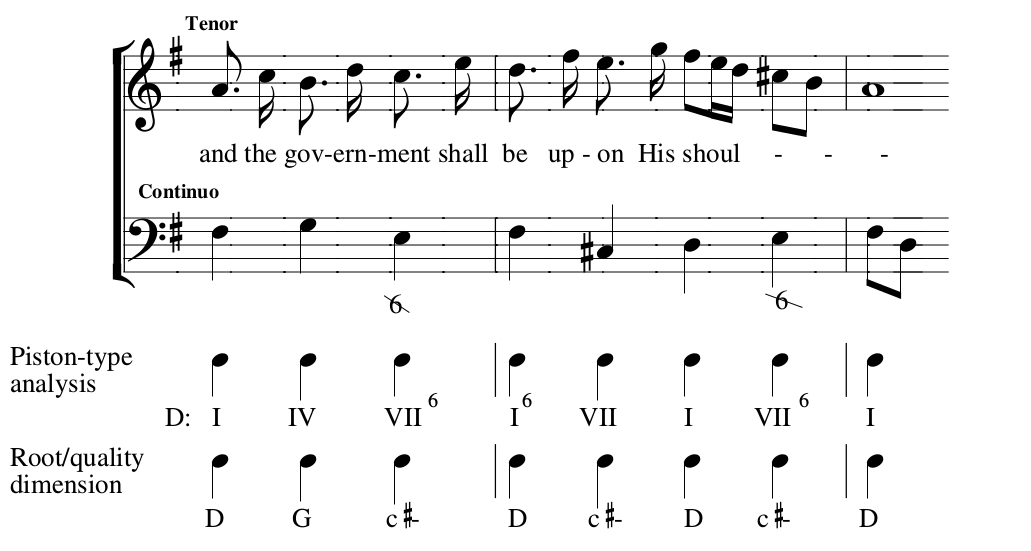
\includegraphics[scale=0.35]{Haendel_Messias_Tenor.jpg}
\caption{Root/Quality harmonic rhythm - G.F. Händel: \textit{Messiah, no. 12 "For unto us"}}
\end{figure}

Thereby, he tries to eliminate the subjectiveness which an analysis needed for functional harmonic rhythm involves. The functional information will be used in the last level of analysis so that no information is lost.

Secondly, Swain introduces a hierarchical system: On the lowest level, all root changes are denoted. On higher levels, brief chords that may be seen as contrapuntal coincidences instead of actual chords, may be omitted and subsumed under a perceptually more important primary chord.\footnote{This idea seems strongly influenced by the Schenkerian idea of hierarchical music analysis, originally put forth by Heinrich Schenker 1906-1935 \cite{schenker1906harmonielehre}, \cite{schenker1991neue} and \cite{schenker1956freie}, and expanded in \cite{jackendoff1983generative}.} Obviously, this type of hierarchical analysis involves a considerable amount of interpretation -- e.g. how many levels to use, how detailed each of these levels should -- reintroducing some of the ambiguity eliminated by using absolute chord symbols instead of Roman numerals. Swain puts forth a number of rules to minimise this ambiguity that I will not further explain here, but may be of interest to the musicologically more inclined reader.\footnote{\cite{swain2002harmonic}, p. 44ff.}

The dimension of root changes or "Quality harmonic rhythm" seems quite suited for the purpose of this thesis: Its independence from tonal systems and subjective opinions by the analyser opens the possibility for broad usage in a range of styles while allowing for post-hoc functional analysis, although limited in detail.

\subsubsection{Density of harmonic rhythm}
On another (though not necessarily more complex) level, Swain considers the chords' density and thus, the strength of the harmonic progression. The density of a progression is defined by the number of voices that change their sounding note into one that is part of the new harmony.\footnote{[ibid.], p.58} While a singular density may not be of high perceptual importance, a passage with high density values will tend to appear more powerful than one with very low density changes, even if they are of the same dynamic force.\footnote{[ibid.], p.60} Again, Swain goes into more detail of the interpretational possibilities and challenges (such as two voices leading into the same note or even the question how to define a voice e.g. in a piano score), that I will not cover here, but may be useful for a deeper understanding.\footnote{[ibid.], p.63ff.}

\subsubsection{Rhythm of harmonic functions}
In the last dimension of his analysis, Swain reintroduces the functional analysis of a piece. While the original idea of Piston used it, the root level probably describes his intentions better. As does Piston, Swain allows for embedding of short phrases that are not long or significant enough to be called an entire modulation.\footnote{[ibid.], p.70ff.} Swain however only uses three symbols (I, IV and V for tonic, subdominant and dominant) since these three basic functions should suffice in his opinion.\footnote{[ibid.], p.69} Thus, he has to use embedding more often than Piston.

\subsubsection{Consequences}
Having seen the two most important works on the topic, it is now time to draw conclusions for the approach of this thesis. While the corpus with which I worked was already finished and the analyses of the pieces had already been made, it is still necessary to check for their validity in respect to harmonic rhythm.

The reductions given to me were on a somewhat inconsistent, but mostly intermediate level of detail. Those pieces that differed from the root level as defined by Swain tended to be of slightly higher precision. From them, analyses were generated by the GCT algorithm, also in work prior to this thesis. The thusly generated chord sequences are, speaking in terms of Swain, of the root change type. As mentioned in the sections above, I consider this level to be a reasonable one for two reasons:

It provides a reasonable tradeoff between feasability and information content as it can be relatively easily generated computationally (as opposed to the highly subjective functional analysis). Other than e.g. the bass movement harmonic rhythm that can contain imprecisions, it yields all of the harmonic information, though not necessarily in an accesible form (i.e. it tracks all harmonic changes, but does not interpret them in a meaningful way).

At the same time, it is usable in non-tonal systems, allowing for a wide range of musical styles to be put into the system. Due to the assumptions made for further analytical steps, I expect a performance bias towards tonal music, since I know best about it and its rules of harmony and harmonic rhythm compared to other idioms.


\section{Aspects of melodies with possible correlations to harmonic rhythm}
In the following section, I will describe the thought process behind the decisions made for some aspects in melodies and my hopes for them being predictors for harmonic rhythm.

\subsubsection{Melodic rhythm}
In his book ``Music and Probability"\footnote{\cite{temperley2007music}}, Temperley puts forth his earlier formulated idea of communicative pressure\footnote{\cite{temperley2004communicative}}: since music has the goal of communicating between composer/interpreter and listener, a common ground of this communication, some kind of ruleset, needs to be set so that the listener has any chance to understand the composer's intentions. This includes style-specific amounts of syncopation and rubato to be used.

Temperley notes that styles with high syncopation tend to be very strict in the tempo used and vice versa. This supports the idea that concurring factors of complexity in music may be negatively correlated. Thus, it seems reasonable to assume that this might also apply to harmonic rhythm and some other feature (e.g. melodic rhythm) in terms of speed and complexity. As it is very hard to properly define ``complexity'' of a melody, I instead used the "Weighted Note-to-Beat distance" (WNBD) syncopation measure as an indicator of rhythmic complexity.\footnote{For the mathematical reasoning and a longer algorithm description, see \cite{gomez2005mathematical}, for a comparison between a number of complexity measures, see \cite{thul2008rhythm} and for experimental evidence, see \cite{fitch2007perception}.}

This algorithm takes each note's distance to the closest strong beat (e.g. the fourths in a 4/4) called $T(x)$. If it is 0, obviously the distance measure is 0. If however, the note is not on a strong beat, there are a few different cases: If the note ends on or before the next strong beat, the distance is $\frac{1}{T(x)}$. If it continues longer than the next beat, but ends on or before the subsequent one, the distance becomes $\frac{2}{T(x)}$. If the note's duration is even longer than that, we return to the first formula $\frac{1}{T(x)}$ again. After all the distances of a bar have been calculated, they are averaged, thus giving the rhythmic complexity or syncopation of a bar.

\subsubsection{Melodic contour}
While concurring features may be negatively correlated, it is also quite possible that other features could conincide, such as perceptually more salient points in a melody and changes in harmony. One possible candidate for such a perceptually relevant feature is melodic contour.\footnote{For original papers, see \cite{thomassen1982melodic} and \cite{dowling1971contour} and for an overview, see \cite{dowling1986music}, p.133ff.} While their work talks about memory tasks (specifically short term memory), only that which is perceived can be memorised, making the jump to salience a small one.\footnote{For a comprehensive overview on music and memory, see \cite{hallam2011oxford}, chapter 10.} Therefore, I checked for a positive correlation of contour changes and harmony changes, resulting in a possible prediction of harmonic rhythm.

\subsubsection{Interval structure}
Not only contour, but also the exact interval structure is of perceptual importance in terms of ease of memorisation, especially long term memory.\footnote{\cite{dowling1986music}, p.138ff.} Thus, this may be another feature to take into account for prediction of structurally relevant points, as there may be ``signal intervals" that more often than others indicate a change in harmony, such as classical dissonances that could not lie in the same harmony in earlier tonal music. Another possibility may be that of a correlation between interval size and probability of harmony change. This latter approach grants independence from the preferred genre, while the first one is focused on western tonal music.





\chapter{Methodology}
The pieces used were:
\vspace{1ex}
\begin{itemize}
	\item{35 Bach chorales}
	\item{9 Beatles songs}
	\item{3 Bossa Nova songs}
	\item{4 choral pieces from the neotonal era (Stravinsky, Debussy and Calalang)}
	\item{2 Hindemith pieces}
	\item{26 Jazz songs}
	\item{7 Rebetika (Greek folk songs)}
	\item{12 Tango pieces}
\end{itemize}
\vspace{2ex}
\par
I discarded the idioms with less than 5 pieces (Bossa Nova, Neotonal music and Hindemith) since results in these probably are based on pure chance.

I ended up using only four factors for determining a likelihood for each onset due to the sparsity of the data. These were:
\vspace{1ex}
\begin{itemize}
	\item{Cooccurences of harmonic and melodic rhythm}
	\item{Contour changes}
	\item{Interval size}
	\item{Rhythmic complexity measured by the WNBD (see 2.3)}
\end{itemize}
\par
\vspace{2ex}
I received the pieces as MusicXML files and together with my supervisor Maximos Kaliakatsos-Papakostas extracted harmonic rhythm, melodic rhythm, pitches, time signatures and grouping information in the form of .csv files. These were separated into patterns that were either one bar long or shortened by a grouping (=cadence). This followed the thought that patterns at cadences should be treated differently since in Western music they have higher priority to receive a harmonic event. However, I did not use this information in the end.

Afterwards, I analysed the pieces and extracted the number of cooccurences of harmonic and melodic rhythm, the WNBD as syncopation measure, the absolute intervals (without direction to have more data points) and the contour defined as changes in direction of the melodic movement.

The syncopation values were put into three bins that I created after taking all syncopation values from all pieces and dividing them into three equal parts. I then used the thresholds between these bins as thresholds for the three categories.

Then, these numbers where used to calculate conditional probabilities for a harmonic event occurring given one of the following nine criteria:
\vspace{1ex}
\begin{itemize}
	\item{Melodic event}
	\item{Contour change}
	\item{Unison in the melody}
	\item{Step in the melody}
	\item{Jump in the melody (everything from third to seventh)}
	\item{Big jump in the melody (octave or larger)}
	\item{Low syncopation ($WNBD \leq 0.5$)}
	\item{Medium syncopation ($0.5 < WNBD \leq 1$)}
	\item{High syncopation ($1 < WNBD$)}
\end{itemize}
\par
\vspace{2ex}
From these conditional probabilities for each idiom, one piece that I left out of the analysis by random choice received a prediction. I did this by iterating over a list of the melody offsets and strong beats as possible time points where harmonic events could occur -- the implications of which will be discussed lateron -- and for each time point calculating the combined probabilities of all the features. For strong beats that had no melodic event occurring on them, I simply took $1 - P(harmonic~event | melodic~event)$.

From this list of likelihoods I chose the highest ones until the target number was reached which I calculated as $(mr * P(harmonic~event|melodic~event) + sb * (1 - P(harmonic~event|melodic~event)))$ with mr as the number of melodic events and sb as the strong beats without melodic events.

I evaluated the results mainly with the Jaccard distance between the sets of predicted harmony offsets and the actual harmony offsets from the original piece. I also had a look at the percentages of correct guesses.

The Jaccard distance is defined as the cardinality of the intersection of two sets divided by the cardinality of the union of these two sets, or as a formula:

{\centering
\Large
$jd = \frac{|P\cap O|}{|P\cup O|}$
\par}
\normalsize


\chapter{Results}
As an example for the conditional probabilities found, here are those for Bach chorales:

\begin{figure}[h]
	\centering
	\begin{tabular}{|l|c|c|c|c|r|}
		\hline
		\textbf{Feature} & Melodic event & Unison & Step & Jump & 		Big jump \\ \hline
		\textbf{Probability} & 0.812 & 0.402 & 0.366 & 0.499 & 0.059 			\\ \hline
	\end{tabular}
	\par
	\vspace{2ex}
	\begin{tabular}{|l|c|c|c|r|}
		\hline
		\textbf{Feature} & Contour & Low WNBD & Medium WNBD & High WNBD \\ 			\hline
		\textbf{Probability} & 0.359 & 0.407 & 0.176 & 0.049 \\ \hline
	\end{tabular}
	\caption{Conditional probabilities for Bach chorales}
\end{figure}
\par
\vspace{1em}

Below are also the Jaccard distances between my predictions and the correct harmony offsets for the test pieces from the five bigger idioms.

\begin{figure}[h]
\centering
	\begin{tabular}{|l|r|}
		\hline
		\textbf{Idiom} & \textbf{Jaccard distance}\\ \hline
		Bach chorales & 0.596 \\ \hline
		Beatles & 0.151 \\ \hline
		Jazz & 0.271 \\ \hline
		Rebetika & 0.1 \\ \hline
		Tango & 0.110 \\ \hline
	\end{tabular}
	\caption{Received Jaccard distances for the test pieces}
\end{figure}
\par
\vspace{1em}

The complete results can be found in the addendum or in my github repository under https://github.com/VHuemerlehner/Bachelors-Thesis

\chapter{Discussion}
\subsection{General}
As can be seen in point 5, the results are not very convincing. One thing to consider in favour of the results is however that the Jaccard distance is quite the conservative measure for my evaluation for two reasons:

First, it does not take the musical implications into account. Whether a harmony is put onto some highly unlikely spot or onto one that is very likely and might result in a pleasant harmonisation is unimportant as long as neither of the spots is in the correct harmonisation.

Second, it is not a measure of similarity to human perception, but a mathematical measure. Most humans would not perceive the difference between a 0.95 and 0.9 rating, I presume. For a predicted harmonic rhythm to be perceived as belonging to an idiom does not necessitate a completely correct prediction, but only one that is similar enough.

\subsection{Positive results}
One positive aspect in the results is also the consolidation of Temperley's theory of communicative pressure in another aspect of music. Similarly to the above shown probabilities for Bach chorales, all idioms except the Rebetika show the same pattern of high syncopation leading to less harmonic events. The intuition of e.g. Jazz being a nice example is found correct in my work.
\vspace{1ex}

\subsection{Critique}
Looking for reasons for the poor results, there is quite a number to find that automatically should be considered possible improvements for future work.

The first problem appeared already in the MusicXML files. Towards the end, I found seemingly minor mistakes that forced me to rethink a step in the prediction process, such as a full 4/4 bar in the grouping voice with all other voices having only 3/4 in that bar and an appoggiatura to the next one. This lead to non-equal overall lengths of the voices and unexpected parsing problems.

A second hiccup happened in the analysis stage where not all pieces were analysed according to the same philosophy: Some counted minor voice movements in the accompaniment as harmonic events, others left those out, meaning that the data collected was not completely consistent in itself.

The third mistake was poor planning on my end, conceptually as well as organisationally. I did not properly note down what happened and which thoughts occured around the proceedings. This lead me to repeat my own thoughts time and time again, hindering actual progress. On the conceptual end, if I had spent more time thoroughly thinking through the steps needed for completion of my predictions, surely not all problems could have been avoided, but some of the more obvious ones and quite some unnecessary work that I did not use in the end could have.

In terms of the implementation, I suspect a systematic error somewhere in the calculation of how many harmonic events should be put as the number is consistently lower than the real one. I was unable to find this error, so it remains a theory and it may have been random that all the pieces I used for predictions had an unusually high amount of harmonic events, but this seems unlikely.

I also suspect, but can not prove, a systematic bias towards Western music. While the Rebetika are not the only idiom with low overall fit, the result strikes me as especially poor due to the contradiction of the theory of communicative pressure. For low syncopation, the Rebetika have a probability of 0.087, for medium syncopation 0.144 and for high syncopation 0.118. This to me seems like a categorical difference between the idioms and thus raises the suspection that the theory put forth in this thesis may only hold for Western music, although further idioms would have to be checked to get more compelling results.

Furthermore, I calculated the syncopation thresholds for all idioms at once. Results may have been clearer -- maybe this was another reason the theory did not work for Rebetika -- if each idiom had received its own syncopation categories.

Lastly, I probably put too many restrictions onto the system that I drew from musical expertise, thus making the algorithm less independent. One example are the possible timings considered for harmonic rhythmic events that conform to Western music standards, but need not be the same in other musical styles.

\subsection{Recommendations and future work}
Stepping away from errors towards suggestions for improvement of the system, my first idea is to use the gathered probabilities not only for the timings were a melodic event occurs, but also on the surrounding ones, since syncopation is not actually a local, but a regional feature. Intervals and contour as well do not only have perceptual importance in the very moment of their occurence, but probably also influence perception in the following time.

As written above, using separate syncopation thresholds for the idioms might help improve the system's performance, hopefully especially the Rebetika.

Overall performance in the idioms I used would probably drop if I reduced the Western bias, but I suspect the Rebetika and other such idioms should profit if less Western expertise and more general features were used in the prediction process.

Lastly, a bigger corpus of pieces would surely help the system achieve better scores, as more different features could be evaluated and the ones that were already used would receive stronger differentiations between one another.

\vspace{1em}
Expanding on this thesis, one could obviously remove some mistakes that happened, but more importantly, a much bigger corpus would be needed not only within the idioms, but also in terms of idiom diversity. While in terms of chronology and styles, the samples are already distributed not too poorly (roughly 1650 - today and from serious to popular music), all except the Rebetika were highly Western idioms. It is a seemingly very general problem in the Western musicology that different styles from other continents are not considered in science and I too am guilty of this shortcoming.

A comparison between the harmonic rhythms of East Asian, Central Asian, Middle Eastern, North African, Sub-Saharan, Australian aboriginal, North American aboriginal and South American styles would require an immense amount of work, but surely would create some interesting results and allow for less biased music producing systems.

Another aspect to consider for future work is blending of the idioms: As the CHAMELEON system is able to blend, so too should be its module for harmonic rhythm. A very na\"{i}ve approach that might work a little bit would to simply average the probabilities of two idioms, however, this would probably result in a loss of many important features. However, without a better performing system, it is difficult to predict where exactly the idiom defining differences will lay.

%END normal LaTex document
\newpage
\pagenumbering{roman}
\bibliographystyle{apalike}
\bibliography{mainbiblio}

\closing
\end{document}